\chapter{Resultados y Análisis}\label{chapter:results}
\newcommand\graphwidth{0.65}

En este capítulo se presentan los resultados y análisis de las validaciones propuestas en el Capítulo \ref{chapter:diseno} y presentadas en el Anexo \ref{appendix:validations}. En primer lugar, se revisa el cumplimiento de las funcionalidades del sistema por medio de pruebas en un robot simulado. Luego, se revisa el estado de la integración en el robot Bender, de acuerdo a las validaciones asociadas. Finalmente, se presentan los experimentos de escalabilidad y eficiencia utilizados para medir el desempeño del sistema LTM implementado.


\section{Funcionalidad del Sistema LTM}

A continuación se presentan los resultados de las validaciones de funcionalidad del sistema LTM. El listado se encuentra en el Anexo \ref{appendix:validations} y consta de 28 validaciones, cada una con el prefijo \Vlabel{A}{XX}. A modo general, cada una busca validar el cumplimiento de requisitos pertenecientes a alguna de las siguientes categorías: reglas episódicas de Stachowicz, generalidad de la implementación y el funcionamiento de las relevancias episódicas.

Para las pruebas se utilizó un robot simulado, de acuerdo a lo presentado en la Sección \ref{sec:impl-validation}. El sistema LTM fue configurado para utilizar el plugin de \textit{streams} de imágenes, el plugin de entidades tipo personas y objeto, y la interfaz episódica para SMACH. Además, los episodios son obtenidos a partir de una máquina de estado implementada mediante SMACH, que simula el flujo de estados utilizados en una prueba de la competencia RoboCup.

\subsection{Generalidad del sistema LTM}

Uno de los énfasis del diseño del sistema LTM es la generalidad del mismo. El objetivo es que el proyecto pueda ser utilizado por otros robots además de Bender, como por ejemplo, Maqui, otro robot del mismo laboratorio. A continuación se describen los conceptos de interés para lograr este objetivo, y cómo se relacionan con las validaciones.

En primer lugar, el sistema LTM soporta la definición de plugins para el manejo de estructuras episódicas de acuerdo a los requerimientos del usuario (\Vlabel{A}{02}). Esto es fundamental para poder utilizar el sistema LTM en cualquier plataforma, pues evita forzar una representación de la información, dejando la adquisición de ésta al usuario.

Además, la implementación fue separada en 3 grupos de paquetes ROS para desacoplar el sistema (\Vlabel{A}{03}). El primero contiene el manejo de la base de datos y la implementación del servidor genérico a base de plugins. El segundo provee el plugin para streams de imágenes y la interfaz episódica para SMACH, ambos son componentes genéricos, pero no son esenciales para el funcionamiento del sistema LTM. El último provee implementaciones de plugins específicos para el robot Bender.

La implementación del servidor sólo requiere un mínimo de dependencias (\Vlabel{A}{16}) y no necesita módulos de Bender para su funcionamiento (\Vlabel{A}{01}). Además, el servidor provee una API ROS para el manejo de episodios (\Vlabel{A}{26,27}).

Todas las validaciones asociadas se pueden verificar a partir de la implementación de plugins para el robot simulado, el que define mensajes episódicos para los streams y entidades que utiliza.

Debido a los puntos anteriores, el sistema LTM implementado se puede ajustar a las necesidades de otros proyectos robóticos, sin requerir software de Bender.


\subsection{Reglas episódicas de Stachowicz}

El otro foco del proyecto está en el cumplimiento de las reglas episódicas propuestas por Stachowicz. A modo de resumen, todas las validaciones asociadas se cumplen, a excepción de \Vlabel{A}{17}. A continuación se describen los conceptos asociados a cada una de las validaciones de interés.

Los episodios son representados por un mensaje ROS con componentes genéricos. El usuario puede definir las estructuras de datos para la información semántica de interés utilizada en el campo \textit{What}: streams y plugins. El campo \textit{When} sólo considera tiempos de inicio y fin, sin imponer restricciones sobre el lapso de tiempo. Además, no existe una restricción temporal entre un episodio y otro, lo que permite generar episodios traspuestos en el tiempo, siempre que uno no sea descendiente del otro. El campo \textit{Where} permite almacenar la posición del robot durante cada episodio, mediante una representación literal o a través de una pose dentro de un sistema coordenado.

La implementación permite recolectar episodios y sus componentes semánticos a partir de consultas en formato JSON, aplicando condiciones booleanas de búsqueda, a través de una API ROS. El diseño soporta la actualización de entidades y la perspectiva episódica de éstas, pudiendo reconstruir el estado de una entidad en distintos instantes de tiempo. Los episodios son únicos y mantienen referencias bidireccionales a las unidades semánticas relacionadas. Los episodios se estructuran a modo de árboles, permitiendo el anidamiento episódico.

Por un lado, todos los puntos anteriores se validan mediante los conceptos descritos en el diseño (Capítulo \ref{chapter:diseno}) y la implementación del sistema LTM (Capítulo \ref{chapter:implementacion}). Por otro lado, de una manera práctica, es posible validar las reglas anteriores mediante la ejecución del sistema LTM para el robot simulado, ejecutando una máquina SMACH para generar episodios, para finalmente realizar consultas episódicas a través del servicio ROS que provee el servidor LTM.
\todoimprove{Código para ejecutar el sistema simulado + consultas interesantes.}

La validación \Vlabel{A}{17} no se cumple. Está relacionada al requisito de sistema \RSlabel{14}, el que indica que el usuario debe poder cambiar la representación del episodio en el futuro, sin sacrificar la información de episodios que utilizan la versión anterior. Particularmente, el usuario debe poder modificar los campos del mensaje ROS de los streams o entidades definidas para sus plugins. Se cree que el diseño soporta esta funcionalidad, pero no fue implementada por falta de tiempo. Queda propuesta la implementación de una funcionalidad capaz de migrar todos los episodios de la base de datos a la nueva representación episódica.

\subsection{Relevancias episódicas}

Se requiere la implementación de la relevancia emocional, histórica y generalizada. A continuación se revisan los puntos necesarios asociados a las validaciones requeridas.

El sistema LTM implementado soporta el concepto de relevancia episódica, almacenando sus datos mediante el mensaje ROS \texttt{ltm/Relevance.msg}, embebido en el mensaje \texttt{ltm/Episode.msg}. Debido a esto, es posible incluir cualquiera de los campos en las condiciones de búsqueda, permitiendo filtrar episodios por cualquiera de las relevancias (\Vlabel{A}{25}).
\todoimprove{Código de ejemplo para filtrar por relevancia.}

La relevancia emocional fue implementada en el mensaje \texttt{ltm/EmotionalRelevance.msg} (\Vlabel{A}{21,22}). Sus datos son recopilados mediante un plugin implementado por el usuario. El paquete \texttt{ltm\_samples} provee un plugin de ejemplo, capaz de adquirir el estado emocional del robot simulado.

En cuanto a la relevancia histórica (\Vlabel{A}{23}), ésta ha sido parcialmente implementada. Utiliza el mensaje ROS \texttt{ltm/HistoricalRelevance.msg} para su representación, pero no se ha implementado la rutina para actualizar automáticamente el indicador de relevancia con el paso del tiempo. Sin embargo, en el Capítulo \ref{chapter:diseno} se describe su diseño y una metodología para su implementación.

Ya que la relevancia histórica aún está incompleta, también se postergó la implementación de la relevancia generalizada (\Vlabel{A}{24}). Asimismo, el capítulo de diseño describe una metodología para su implementación y actualización.

Tanto la relevancia histórica como la generalizada pueden ser consideradas parte del trabajo futuro, donde sólo queda implementar el algoritmo de actualización.


\subsection{Revisión}

A modo de resumen, el foco del proyecto estuvo en el diseño e implementación de un sistema LTM genérico, basado en las reglas episódicas de Stachowicz. El objetivo fue diseñar un sistema LTM para el robot Bender, pero que pueda ser integrado en otras plataformas robóticas. Las validaciones asociadas a estos conceptos se cumplen todas, a excepción de \Vlabel{A}{17}, relacionada con la migración de la base de datos al modificar la representación episódica.

En cuanto a las relevancias episódicas, sólo queda pendiente la implementación del algoritmo para la actualización automática de la relevancia histórica y la genérica.

Luego, las únicas validaciones de funcionalidad pendientes son: \Vlabel{A}{17}, \Vlabel{A}{23} y \Vlabel{A}{24}.


\section{Integración en Bender}

A continuación se describe es estado de la integración del sistema LTM en el robot Bender. Las 6 validaciones de interés se presentan en el Anexo \ref{appendix:validations}.

Durante el periodo de implementación del proyecto, incluso hasta la fecha, el robot Bender no ha estado operativo. El equipo encargado ha decidido reestructurar el hardware del robot y además, está en el proceso de migrar URF a ROS kinetic. Por lo anterior, se ha retrasado la integración del sistema LTM en el robot y sólo algunos de los componentes requeridos se han integrado.

La integración requiere la implementación de plugins para el sistema LTM, la generación de episodios a partir de las máquinas de estado del robot y la integración de tal código en URF.

\subsection{Módulos integrados en URF}

A continuación se describen los componentes integrados en Bender. Estos corresponden a piezas de software que no requieren el uso del robot para su integración, o son suficientemente genéricos como para utilizar una versión simulada.

\ltmconcept{Plugin para streams} Debido al diseño genérico del plugin para la recolección de streams de imágenes, este componente fue integrado mediante la selección del tópico ROS de la cámara de video del robot.

\ltmconcept{Plugin de para campo \textit{Where}} Se creó un plugin para la recolección de la ubicación del robot según las consideraciones de diseño descritas en el capítulo \ref{chapter:diseno}. Esta integración fue posible, debido a que Bender utiliza un conjunto estándar de paquetes ROS para navegación robótica (ROS navigation stack). Su funcionamiento fue verificado mediante la simulación de un robot que utiliza estos paquetes para navegar y localizarse.

\ltmconcept{Interfaz LTM-SMACH} Según se presentó en el Capítulo \ref{chapter:results}, la interfaz del sistema LTM con las máquinas de estado en SMACH se implementó de manera genérica y funciona de acuerdo a los requerimientos. Para validar esta integración, se implementó una máquina de estado similar a una prueba de la competencia RoboCup, con la que el sistema LTM puede recolectar episodios.

\ltmconcept{Integración en URF} Todos los componentes descritos anteriormente fueron integrados en URF mediante el paquete ROS \texttt{bender\_ltm}. El proceso de instalación fue modificado para incluir los paquetes ROS del sistema LTM y la instalación de sus dependencias. Se añadieron archivos \texttt{launch} y de configuración para ejecutar el sistema LTM con los plugins integrados.

\subsection{Módulos pendientes}

A continuación se describen los componentes que no se han integrado al software del robot. Estos corresponden al plugin para recolección de entidades y al plugin emocional.

\ltmconcept{Plugin para entidades} Según se describió en la Sección \ref{sec:design_bender}, se debe implementar un plugin para la recolección de entidades tipo persona y objeto, a partir de los módulos de percepción del robot. Este plugin no se ha desarrollado.

\ltmconcept{Plugin emocional} Este plugin no ha sido implementado por dos razones. Como se explicó anteriormente, no se pudo acceder al robot para la integración. Sin embargo, el problema de fondo es que Bender no dispone de un motor emocional, capaz de generar emociones a través de los estímulos que percibe. La implementación de un sistema emocional escapa del alcance del proyecto. Sin ese requerimiento es imposible implementar el plugin requerido.

Por lo tanto, la integración del sistema LTM en Bender es parcial. Queda propuesta la implementación del plugin para entidades, el motor emocional para el robot y el plugin asociado.

\subsection{Demostración del sistema en Bender}

Uno de los objetivos específicos del proyecto es la integración del sistema en el robot Bender y la posterior generación de una demostración de tal funcionalidad. Ya que no se dispone de robot, no se ha podido concretar este objetivo. 

Una vez integrados los módulos pendientes, se debe ejecutar una máquina de estado en SMACH para la recopilación de episodios con información semántica sobre personas y objetos. Luego, el robot debe responder a un conjunto de preguntas sobre hechos pasados mediante el servicio de consultas que provee el sistema LTM.


\section{Desempeño del Sistema}

A continuación se presentan los resultados para las validaciones de eficiencia y escalabilidad definidas en el Capítulo \ref{chapter:diseno}, cuyo objetivo es medir el desempeño del sistema para un conjunto de consultas de interés. En primer lugar, se describen los procesos a ser estudiados y la máquina objetivo. Luego, se identifica el conjunto de operaciones de lectura y escritura a ser utilizado para la evaluación. Tercero, se hace una estimación sobre la cantidad de episodios y la tasa de consultas a evaluar según el caso de estudio. Más adelante, se presenta la metodología de medición utilizada, para finalmente, presentar los resultados y análisis de las pruebas realizadas.

\subsection{Consideraciones}

En esta sección se evalúa el desempeño del sistema LTM, de acuerdo a las validaciones \Vlabel{C}{X} presentadas en el Anexo \ref{appendix:validations}.

\ltmconcept{Procesos}
Una vez activo, el sistema LTM se compone de dos procesos ejecutados simultáneamente en la máquina objetivo. Por un lado, se ejecuta el proceso correspondiente al servidor LTM (en adelante, LTMp), encargado de procesar las consultas ROS, ejecutar los plugins definidos por los usuarios y de mantener la consistencia de la base de datos. Por otro lado, se requiere que el servidor de MongoDB (en adelante MongoDBp) esté activo para responder a las consultas del LTMp. En adelante, se hará la distinción entre LTMp y MongoDBp al hablar de las validaciones a realizar. Además, se hablará de \textit{sistema LTM} para referirse a la combinación de ambos procesos.

La distinción anterior es importante, pues permitirá entender donde se encuentran los puntos críticos donde el procesamiento se estanca e identificar las responsabilidades de cada proceso. Además, se considera necesario enfatizar que todas las consultas de lectura en el sistema LTM son entregadas directamente a la librería de MongoDB para C++, utilizada por LTMp, por lo que se espera que el mayor costo de recursos se atribuya a MongoDBp, a tal librería y al formato de las consultas. Por otro lado, se espera que LTMp incremente el uso de recursos, de acuerdo a la cantidad de plugins utilizados y la calidad de su implementación.

Finalmente, tanto LTMp como MongoDBp son procesos que sólo ocupan 1 núcleo de la máquina en donde residen. Por lo tanto, en el peor caso, las pruebas de eficiencia indicarán el uso de dos núcleos del CPU. Sin embargo, es posible que algunos plugins LTM, implementados por el usuario, requieran del uso de más de 1 núcleo.

\ltmconcept{Especificaciones de la máquina} En el caso de Bender, URF se ejecuta en 3 computadores simultáneamente. A pesar ésto, las pruebas se realizaron en sólo uno de los computadores, el que tiene las siguientes especificaciones de interés:
\begin{itemize}
%\item Modelo: 
\item CPU: Intel(R) Core(TM) i5-2500K CPU @ 3.30GHz
\item RAM: 15.6 GB
%\item Disk IO:
\end{itemize}


\subsection{Consultas de interés}

De acuerdo a lo revisado en la sección \ref{sec:data_model_design}, las operaciones CRUD más relevantes son las de creación y lectura de episodios.

\ltmconcept{Inserción de episodios}
La operación de creación se realiza en un proceso de dos etapas, registro e inserción. Durante el registro, LTMp se encarga de generar un identificador único para el episodio y avisar a los plugins. Éste proceso es rápido y no se considera necesario realizar una medición de su impacto en el sistema. Por otro lado, la etapa de inserción se encarga de actualizar el árbol episódico y de almacenar los cambios en la base de datos. Este proceso puede ser costoso y se considera interesante para el estudio.

Luego, la consulta de interés es la de inserción de episodios, la que se realiza a través del servicio ROS \texttt{$\sim$/ltm/episode/add}. En los gráficos de resultados esta operación siempre se presentará mediante una línea negra, marcada con símbolos \texttt{+} por cada muestra obtenida.

\ltmconcept{Búsqueda de episodios}
Asimismo, la operación de lectura de episodios se realiza a través de un proceso de dos etapas, búsqueda en la base de datos y recopilación de documentos con los episodios de interés. En este caso, la operación de interés es la de búsqueda de episodios dada una consulta expresada mediante distintas condiciones booleanas. Según la cantidad de episodios y las condiciones de búsqueda, esta consulta puede ser más o menos costosa.

Luego, la consulta de interés es la de búsqueda de episodios, la que se realiza a través del servicio ROS \texttt{$\sim$/ltm/db/query}. Las condiciones de búsqueda se expresan en formato JSON, siguiendo la sintaxis para consultas utilizado por MongoDB.

Ya que las condiciones de búsqueda pueden afectar el desempeño del sistema, se define un conjunto de 5 consultas JSON, con el fin de evaluar el sistema LTM bajo distintos casos de uso. Las consultas se presentan en el Código \ref{lst:validation-queries} y se describen a continuación:
\begin{itemize}
	\item $Q_1$: Consulta que filtra episodios a partir de una condición de igualdad entre un campo y un valor numérico de tipo entero.
	\item $Q_2$: Consulta que filtra episodios donde un valor particular se encuentra dentro de un campo de tipo lista de \textit{string}.
	\item $Q_3$: Consulta que filtra episodios donde un campo de tipo \textit{string} coincide con alguno de los que se provee en la lista que se provee.
	\item $Q_4$: Consulta que filtra episodios mediante dos condiciones unidas por el operador lógico OR. Una de las consultas evalúa una condición de orden (mayor qué) para un valor de tipo decimal. La otra consulta es idéntica a $Q_2$.
	\item $Q_5$: Consulta que filtra episodios mediante 3 condiciones de búsqueda, anidadas por operadores lógicos OR y AND. Las consultas internas son similares a $Q_2$ y a la de orden utilizada en $Q_4$.
\end{itemize}
En adelante, se referirá a cada consulta por su abreviación en el formato $Q_x$, donde $x$ corresponde al número de la consulta presentado anteriormente. En los gráficos, se utilizará siempre el mismo color y estilo de línea para representar a una misma consulta.

\lstset{style=/Style/JSON}
\lstinputlisting[caption=Consultas JSON utilizadas para validación,label=lst:validation-queries]{code/json/validationQueries.json}


\subsection{Estimaciones}

Para poder ejecutar las validaciones de escalabilidad y eficiencia es necesario conocer el uso esperado del sistema LTM en el robot objetivo. Acá se presentará una estimación del orden de magnitud para la cantidad de episodios y la tasa de consultas necesarias para las validaciones, dado un caso de uso esperado.

\ltmconcept{Caso de uso}
El robot objetivo de este proyecto es Bender, el que se entiende como un robot de laboratorio, con un tiempo de operación diario muy bajo. Se tienen las siguientes consideraciones:
\begin{itemize}
\item El equipo suele trabajar solamente en los tiempos libres durante los días de clases. Es decir, 5 días a la semana, durante 32 semanas de clases al año.
\item El robot no es utilizado todos los días, sino que de manera intermitente, siendo encendido por cortos periodos de tiempo.
\item De las veces que el robot está en funcionamiento, sólo muy pocas veces se encuentra ejecutando una máquina de estado.
\end{itemize}

Por lo anterior, los requerimientos impuestos para las validaciones son bajos. Sin embargo, es deseable que el sistema LTM sea capaz de soportar una carga más exigente de episodios y consultas, por el ejemplo, asumiendo que el robot funciona durante todo el horario laboral de manera ininterrumpida.

\ltmconcept{Cantidad de episodios}
Según el caso de uso esperado, se hace una estimación de la cantidad de episodios a recolectar, para soportar el uso del sistema LTM de manera continua durante un periodo de 1, 5 y 10 años. 

Para determinar la cantidad de episodios, se estima que en una hora el robot es capaz de realizar 3 sesiones de trabajo. Por cada sesión, se almacena un árbol con 20 episodios. 

En la Tabla \ref{table:escalabilidad} se presentan los valores de cada concepto utilizado para la estimación. Se debe enfatizar que los valores seleccionados son sólo válidos para este estudio y la cantidad real de episodios dependerá del uso dado al sistema LTM.

\begin{table}[H]
	\centering
	\begin{tabular}{|l|c|}
		\hline
		\rowcolor{gray!50}
		Concepto & Valor Estimado \\ \hline
		Semanas / Año	&  32 \\  \hline
		Días / Semana	&  5 \\  \hline
		Horas / Día     &  3 \\  \hline
		Árboles / Hora  &  3 \\  \hline
		Episodios / Árbol & 20 \\  \hline \hline
		Episodios en 1 año  & 28.800  \\  \hline 
		Episodios en 5 años  & 144.000  \\  \hline 
		Episodios en 10 años  & 288.800  \\  \hline 		
	\end{tabular} 
	\caption[Estimaciones para validación de escalabilidad]
	{\small Estimación de la cantidad de episodios necesarios para las evaluaciones de escalabilidad, bajo el caso de uso del sistema LTM en el robot Bender.}
	\label{table:escalabilidad}
\end{table}


\ltmconcept{Cantidad de consultas por minuto}
La cantidad de consultas por minuto esperadas para el sistema LTM, en adelante \textit{CPM}, dependerá mucho del uso del robot. A continuación se hace una estimación gruesa sobre las CPM requeridas para las operaciones de inserción y búsqueda de episodios, se acuerdo a la experiencia que el autor tiene con el robot.

Para el caso de la inserción de episodios, siguiendo las estimaciones de escalabilidad, con 3 árboles/hora y 20 episodios/árbol se estima 1 CPM para consultas de inserción. Sin embargo, es posible que los procesos de inserción se ejecuten de manera consecutiva en un corto intervalo de tiempo, por lo que se propone un valor de 60 CPM.

Para el caso de las búsquedas, la tasa de consultas depende completamente del uso que le de el desarrollador. A modo de experimento, se asumirá que es deseable una tasa de 10 consultas por segundo, es decir, 600 CPM. Sin embargo, una tasa de 10 CPM puede ser aceptable en la mayoría de los casos, asumiendo que el robot debe responder consultas realizadas por un humano durante una conversación.

\subsection{Metodología de medición}

A continuación se detalla la metodología para la generación de episodios, consultas y la medición de las variables de interés para las validaciones requeridas.

\ltmconcept{Generación de episodios}
Tanto las validaciones de escalabilidad como las de eficiencia requieren que la base de datos ya contenga un conjunto de árboles con episodios. La estrategia utilizada es la siguiente:
\begin{enumerate}
\item Se crea una base de datos vacía para cada prueba.
\item Se inserta un árbol de 20 episodios (tamaño esperado). El árbol es de profundidad 3, tiene 1 raíz, 3 nodos internos y 6 hojas. Todos los episodios son generados con campos aleatorios para cada tipo de dato requerido.
\item Según se requiera se repite el paso 2, hasta obtener un árbol del tamaño deseado.
\end{enumerate}
% sobre que el uso de streams y entidades extra agrega complejidad
% Siempre se podrían validar más cosas. No busca ser una validación extensiva, sino que una que se adecúe a los requisitos del robot objetivo.
\todowrite{ERROR: CANTIDAD DE ELEMENTOS DEL ÁRBOL A INSERTAR.}

\ltmconcept{Generación de consultas}
Con el fin de evitar sesgar las mediciones por motivos del caché de búsqueda, los valores de cada campo de las consultas $Q_x$ son generados al azar.  Todos los valores generados corresponden al rango de valores posibles para el campo en cuestión. Por ejemplo, para el campo \texttt{children\_tags}, los episodios generados contienen valores del conjunto $\{ tag_1,\ldots, tag_{1000} \}$, entonces la consulta $Q_2$ sólo utilizará valores al azar obtenidos desde el conjunto correspondiente. Para cada campo se tienen al menos 100 valores y a lo más 1000 valores posibles.

\ltmconcept{Escalabilidad}
Las validaciones de escalabilidad buscan medir el tiempo promedio que toma una consulta en ser ejecutada. Para esto, cada consulta es repetida 100 veces, donde se mide el tiempo que el programa queda bloqueado durante la llamada al servicio ROS correspondiente. Las mediciones son repetidas cada intervalos de 10.000 episodios ingresados al sistema LTM.

Además, se mide la cantidad de memoria secundaria requerida para soportar los episodios en la base de datos. Para esto, se realiza una consulta a MongoDB mediante la librería \texttt{pymongo 3.6.1} para Python 2.7. Todos los valores se obtienen través del comando \texttt{dbStats}\footnote{En MongoDB, el comando \texttt{dbStats} permite obtener estadísticas generales de la base de datos. Más información en la página oficial: \url{https://docs.mongodb.com/manual/reference/command/dbStats/}}. Se realizan las siguientes mediciones:
\begin{itemize}
\item Uso total de memoria secundaria. Se obtiene del commando \texttt{dbStats.fileSize}.
\item Espacio total reservado para documentos, es decir: episodios, streams y entidades. Se obtiene del commando \texttt{dbStats.storageSize}.
\item Espacio utilizado por los episodios. Se obtiene del commando \texttt{dbStats.dataSize}.
\item Espacio utilizado para el indexado de los documentos. Se obtiene del commando \texttt{dbStats.indexSize}.
\end{itemize}

\ltmconcept{Eficiencia}
Las validaciones de eficiencia buscan medir el uso de recursos del sistema (CPU y RAM) al variar las CPM, dada una base de datos con una cantidad fija de episodios. De la misma forma, cada consulta es repetida al menos 5 veces y durante al menos 1 minuto. Además, la medición del uso de recursos se realiza cada 3 segundos, para obtener el promedio de las muestras medidas. Para mantener las CPM, el programa de medición es pausado tras cada consulta, durante el tiempo requerido para mantener la tasa de consultas deseada.

La mediciones sobre el uso de CPU y RAM para cada proceso fueron obtenidas utilizando la librería \texttt{psutil 3.4.2}\footnote{La librería \texttt{psutil} permite el monitoreo de procesos y del sistema en múltiples sistemas operativos. Más información en su web oficial: \url{https://pypi.org/project/psutil/}} para Python 2.7.


\subsection{Validaciones de Escalabilidad}

A continuación se presentan los resultados de las mediciones de escalabilidad y el análisis relacionado a cada uno. Estas mediciones buscan medir los costos temporales de las operaciones y el uso de memoria secundaria, según la cantidad de episodios almacenados en el sistema LTM.

\ltmconcept{Ejecución de mediciones} Se implementó un nodo ROS para las mediciones de escalabilidad del sistema LTM. Este se encarga de crear la base de datos, generar episodios, consultas y realizar las mediciones. El nodo almacena los resultados en un archivo en formato CSV. El nodo se puede ejecutar mediante el siguiente comando: \texttt{\$ rosrun ltm\_samples scalability\_test.py}.

A partir de los resultados, un nodo ROS es utilizado para la generación de los gráficos presentados. Puede ser ejecutado mediante el siguiente comando:
\texttt{\$ rosrun ltm\_samples graphs\_scalability.py}.

\ltmconcept{Muestras recopiladas}
Según se estimó, para un lapso de 10 años el robot Bender recopilaría cerca de 288.800 episodios. Para establecer un factor extra de seguridad en la estimación, se realizaron mediciones con hasta 500.000 episodios, por lo que cada gráfico está compuesto de 50 muestras.

\ltmconcept{Uso de memoria secundaria} Los resultados son presentados en el gráfico de la Figura \ref{result:scalability_disk_usage}.  Por un lado, se ve que el espacio total de memoria secundaria utilizado por MongoDB, es reservado en porciones cada vez mayores. Por otro lado, del espacio reservado, la porción utilizada para el almacenamiento de episodios e índices crece de manera lineal, respecto a la cantidad de episodios almacenados.

\begin{figure}[!ht]
	\centering
	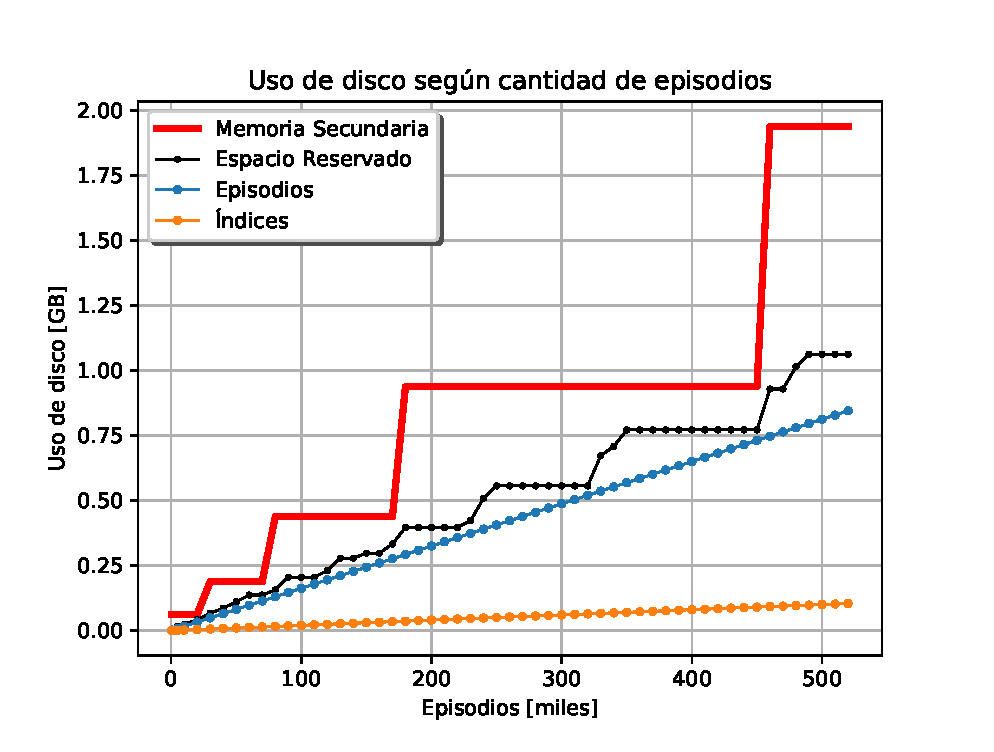
\includegraphics[width=\graphwidth\textwidth]{results/scalability_disk_usage.eps}
	\caption[Escalabilidad: Uso de disco según cantidad de episodios.]
	{\small Prueba de escalabilidad sobre el uso de memoria secundaria  según la cantidad de episodios en la base de datos.}
	\label{result:scalability_disk_usage}
\end{figure}


En sus inicios, el sistema LTM utiliza hasta 0.5 GB para almacenamiento, mientras que a los 10 años (300.000 episodios) llega a utilizar 1 GB en documentos, indices y espacio reservado. 

Se considera que tal cantidad de memoria secundaria no es un problema para las cantidades de espacio disponibles en los computadores actuales. Sin embargo, esta evaluación sólo considera el almacenamiento de episodios, sin streams ni las entidades asociadas. Se espera que el uso de disco aumente de acuerdo a los tipos de dato definidos por el usuario para cada uno de los plugins. 

Particularmente, en el caso de los streams, si se almacenan imágenes en alta resolución a una alta frecuencia, es esperable que el consumo de memoria secundaria sea mucho mayor al mostrado en este experimento. En el caso de las entidades, si éstas no contienen imágenes u otros datos binarios, es esperable que tengan un comportamiento similar al de los episodios.

% Disco utilizado no es un problema. Pero se espera que el espacio aumente según se consideran streams y entidades. Para el caso de 1 stream, con 10 imágenes por episodios, cada una de tamaño AxB, y peso NkB, el tamaño total será ...

\todoimprove{Poner línea sobre el gráfico, indicando los 1, 5 y 10 años}

\ltmconcept{Duración de consultas} Los resultados son presentados en los gráficos de la Figura \ref{result:scalability_time_usage}. Ambos gráficos presentan las mismas mediciones y sólo difieren en la escala y límites del eje temporal.

\begin{figure}[!ht]
	\centering
	\begin{subfigure}[b]{\graphwidth\textwidth}
		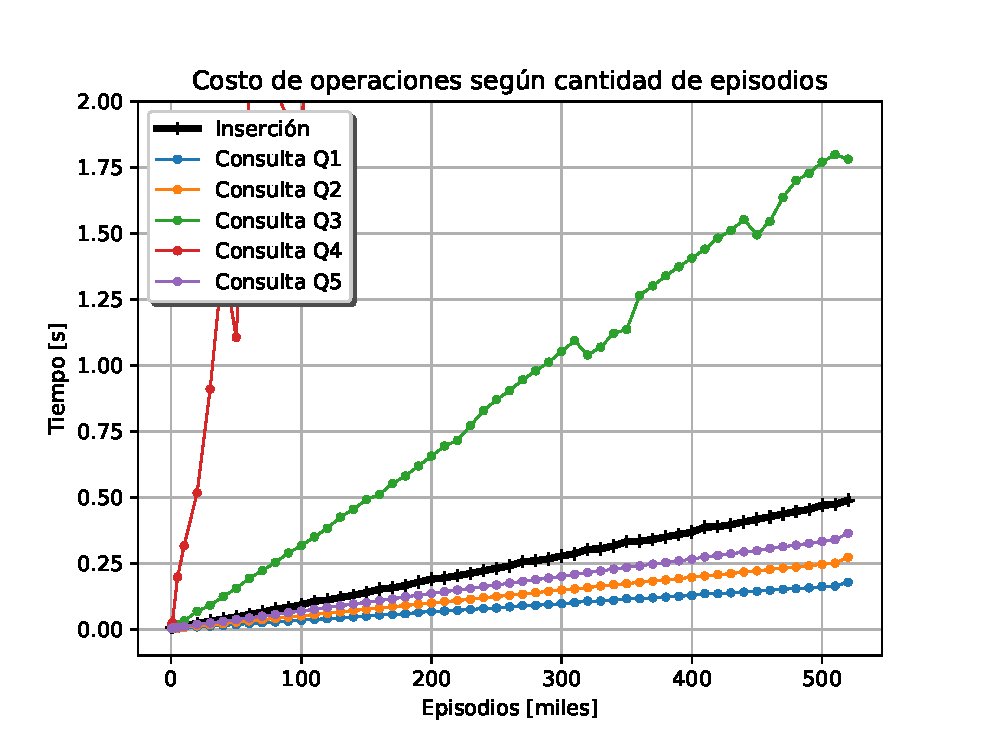
\includegraphics[width=\textwidth]{results/scalability_operation_time.eps}
		\caption{}
		\label{result:scalability_time_usage_normal}
	\end{subfigure}
	~
	\begin{subfigure}[b]{\graphwidth\textwidth}
		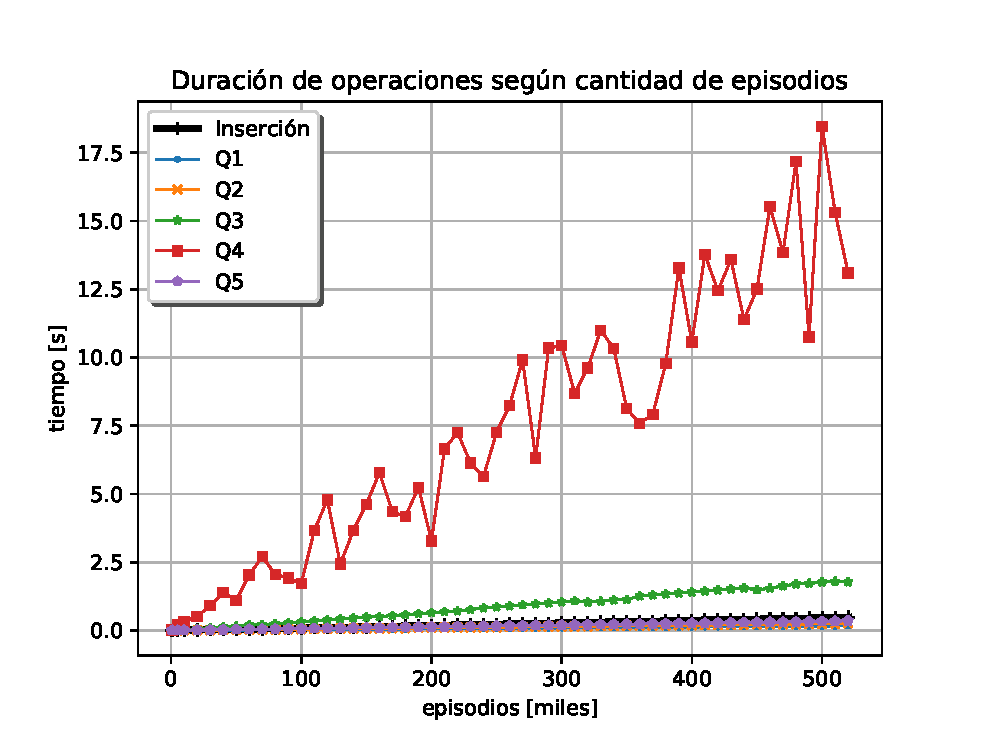
\includegraphics[width=\textwidth]{results/scalability_operation_time_extended.eps}
		\caption{}
		\label{result:scalability_time_usage_extended}
	\end{subfigure}
	\caption[Escalabilidad: Duración de consultas según cantidad de episodios.]
	{\small Prueba de escalabilidad sobre la duración de las operaciones de inserción y búsqueda de episodios en la base de datos según la cantidad de episodios almacenados. Ambos gráficos presentan las mismas mediciones, pero para distintas escalas del eje temporal.}
	\label{result:scalability_time_usage}
\end{figure}

En el caso de la inserción, se puede ver que el costo temporal crece de manera lineal respecto a la cantidad de episodios almacenados. A los 300.000 episodios la consulta requiere alrededor de 0.25[s], mientras que a los 500.000 la consulta toma 0.5[s]. Dado los costos descritos, se impone una cota inferior para la duración de los episodios a generar, pues no será posible almacenar una secuencia de episodios de 0.1[s] cada uno, cuando el sistema LTM requiere más tiempo para su procesamiento. De todas formas, el costo temporal de la inserción es considerado bajo para el caso de uso de Bender.

Para el caso de la búsqueda, se puede ver que todas las consultas, a excepción de $Q_4$, tienen un costo temporal que crece de manera lineal  respecto a la cantidad de episodios almacenados. Las consultas $Q_1$, $Q_2$ y $Q_5$ siempre se mantienen bajo los 0.25[s], mientras que $Q_3$ tiene un costo de 1.0[s] a los 300.000 episodios. En cuanto a $Q_4$, se podría decir que el costo se comporta de manera lineal, pero las mediciones toman demasiado tiempo en ser ejecutadas y tal vez se requieran más muestras para obtener un valor promedio menos variable. Además, $Q_4$ toma 10[s] a los 300.000 episodios, 10 veces más que $Q_3$ y cerca de 40 veces más que $Q_1$, $Q_2$ y $Q_5$.

De lo anterior se puede ver que distintas consultas tienen costos de búsqueda muy  distintos, los que pueden llegar a degradar el funcionamiento del robot, como es el caso de $Q_4$.  Se cree que se debe estudiar en más detalle el costo de todas las operaciones disponibles en el lenguaje de consulta de MongoDB y su interacción con los operadores lógicos, para así disponer de medidas empíricas sobre las cuales diseñar consultas de menor costo.

En cuanto al impacto en la interacción humano robot, es esperable que Bender tenga un funcionamiento ininterrumpido. En este caso, una demora de 0.5[s] en la inserción o búsqueda de episodios puede no ser problema, mientras que en el caso de la consulta $Q_4$, una demora de 10[s] puede comprometer el interés y las expectativas del humano con quien se interactúa. Por lo tanto, en el caso de realmente requerir una consulta compleja como lo es $Q_4$, se recomienda avisar a la persona que el robot deberá procesar la consulta (o ``pensar'') durante unos segundos, para así evitar comprometer la interacción.


\ltmconcept{Límite para las CPM} Finalmente, a partir de los costos en tiempo para cada operación, revisados en la Figura \ref{result:scalability_time_usage}, se puede calcular la tasa máxima de CPM para cada una de las operaciones. Los resultados se presentan en el gráfico de la Figura \ref{result:scalability_max_qpm}. 

\begin{figure}[!ht]
	\centering
	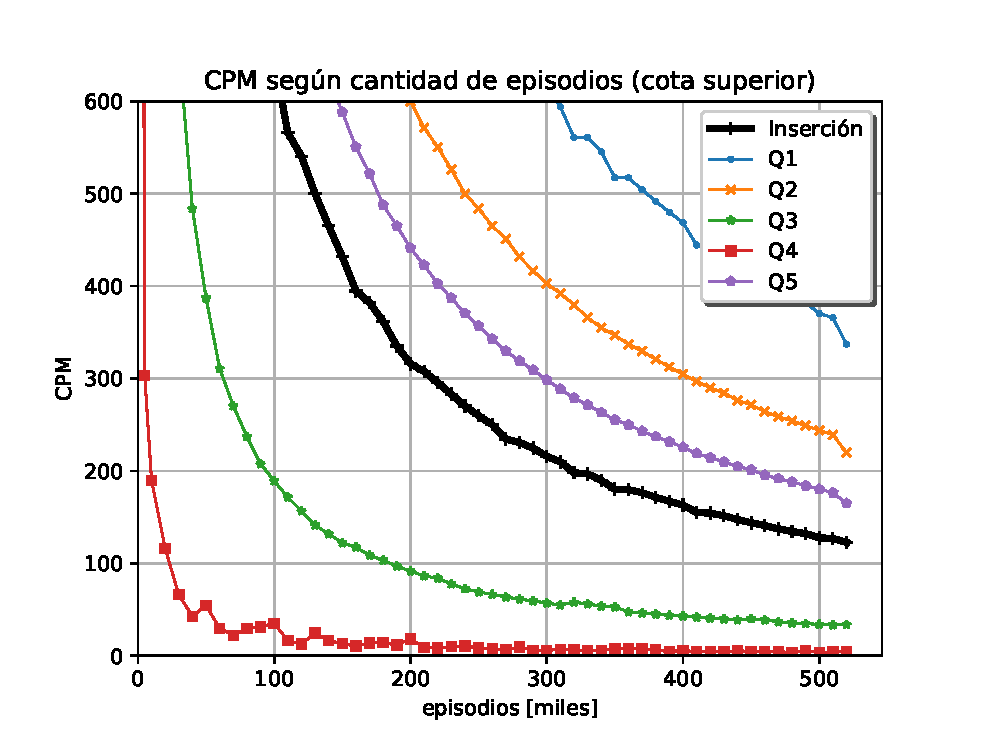
\includegraphics[width=\graphwidth\textwidth]{results/scalability_max_qpm.eps}
	\caption[Escalabilidad: Cota superior para las CPM de cada operación.]
	{\small El gráfico muestra la cota superior para las CPM posibles para cada operación según la cantidad de episodios almacenados en la base de datos.}
	\label{result:scalability_max_qpm}
\end{figure}

Estos resultados son importantes para entender como decrece la tasa de CPM a medida que aumenta la cantidad de episodios almacenados. Además, sirven para comprender el comportamiento de los resultados de eficiencia para distintas cantidades de episodios.



\subsection{Validaciones de Eficiencia}

A continuación se presentan los resultados de las mediciones de eficiencia y el análisis relacionado a cada uno. Estas mediciones buscan medir el uso de RAM y de CPU según la cantidad de consultas por minuto (CPM) a efectuar.

\ltmconcept{Ejecución de mediciones} Se implementó un nodo ROS para las mediciones de eficiencia del sistema LTM. Este se encarga de crear la base de datos, generar episodios, consultas y realizar las mediciones. El nodo almacena los resultados en un archivo en formato CSV. El nodo se puede ejecutar mediante el siguiente comando: \texttt{\$ rosrun ltm\_samples efficiency\_test.py}.

A partir de los resultados un nodo ROS es utilizado para la generación de los gráficos presentados. Puede ser ejecutado mediante el siguiente comando:
\texttt{\$ rosrun ltm\_samples graphs\_efficiency.py}.

\ltmconcept{Presentación de resultados}
En estos experimentos se mide el uso de recursos según la cantidad de CPM utilizadas para distintas cantidades de episodios. Además, ya que se tienen 5 operaciones de búsqueda ($Q_1,\ldots,Q_5$), los resultados se dividirán en dos conjuntos. Primero, se presentan gráficos con una cantidad fija de episodios y los resultados para cada operación. Segundo, se presentan gráficos particulares para cada consulta, con curvas para distintas cantidades de episodios. Finalmente, ya que existen dos procesos de interés, cada conjunto muestra el uso de recursos de MongoDBp, LTMp y del sistema LTM (suma de MongoDBp y LTMp).

\ltmconcept{Muestras recopiladas}
En este caso se presentan mediciones con hasta 100.000 episodios. En cuanto a las CPM, se estimó que se requieren hasta 600 CPM, pero para establecer un factor extra de seguridad en la estimación se realizaron mediciones con hasta 1000 CPM, espaciadas cada 25 CPM. Por lo tanto, cada gráfico dispone de 40 muestras.


\ltmconcept{Uso de RAM según CPM}
Se midió el uso de RAM según la cantidad de CPM para distintas cantidades de episodios y para cada consulta. De los resultados se observó que el uso de RAM no es afectado por la consulta efectuada ni la cantidad de CPM, sino que sólo por la cantidad de episodios. El gráfico correspondiente se presenta en la Figura \ref{result:eff__ram_qpm}, el que representa a todas las consultas evaluadas.

\begin{figure}[!ht]
	\centering
	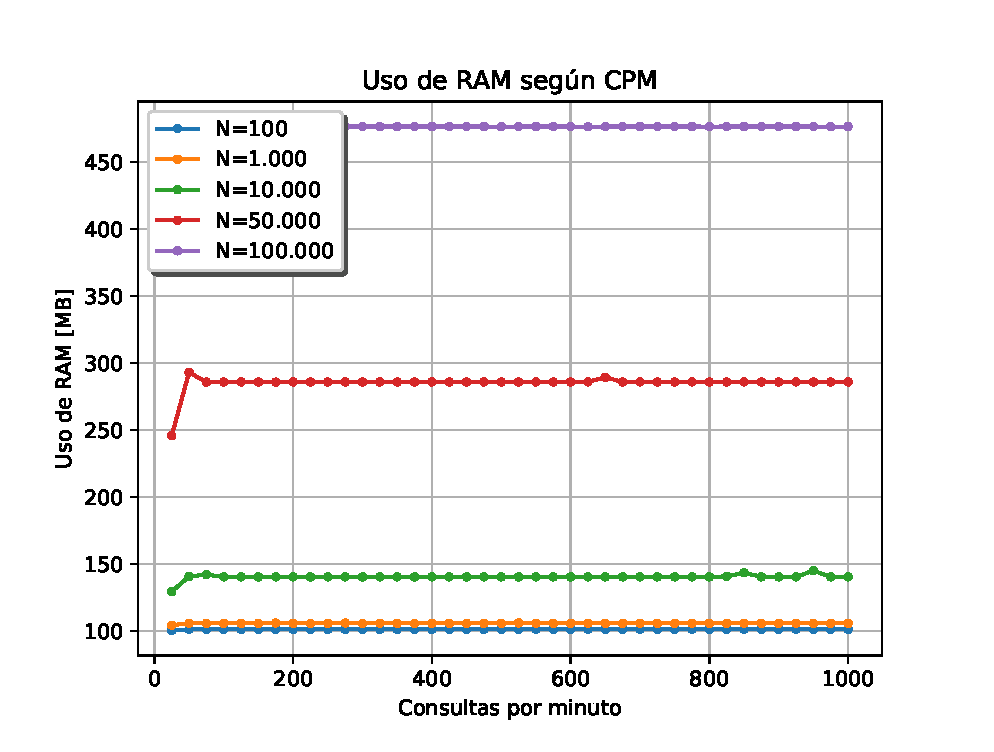
\includegraphics[width=\graphwidth\textwidth]{results/eff__ram_qpm.eps}
	\caption[Eficiencia: Uso de RAM según CPM, cantidad variable de episodios.]
	{\small Prueba de eficiencia sobre el uso de RAM según la cantidad de CPM, para distintas cantidades de episodios. Los resultados presentados son independientes de la consulta efectuada.}
	\label{result:eff__ram_qpm}
\end{figure}
\todowrite{Medidas LTMp, MongoDBp o sistema LTM?}

De los experimentos se entiende que el consumo de RAM debe ser visto como parte de las medidas de escalabilidad y no de eficiencia. Para los 100.000 episodios (alrededor de 5 años de uso) el sistema LTM consume aproximadamente 500 MB de RAM. Sin embargo, se cree necesario conocer la curva de escalabilidad del consumo de RAM, para poder entender el uso de recursos en mayor detalle.


\ltmconcept{Uso de CPU según CPM, cantidad fija de episodios} En la Figura \ref{result:eff__cpu_qpm_by_query} se presentan 6 gráficos con las mediciones de eficiencia del uso de CPU según la cantidad de CPM, para cada consulta y manteniendo fija la cantidad de episodios. Se hace una separación por cada proceso y la suma de ambos, y para 10.000 y 100.000 episodios.

\begin{figure}[!ht]
	\centering
	\begin{subfigure}[b]{0.45\textwidth}
		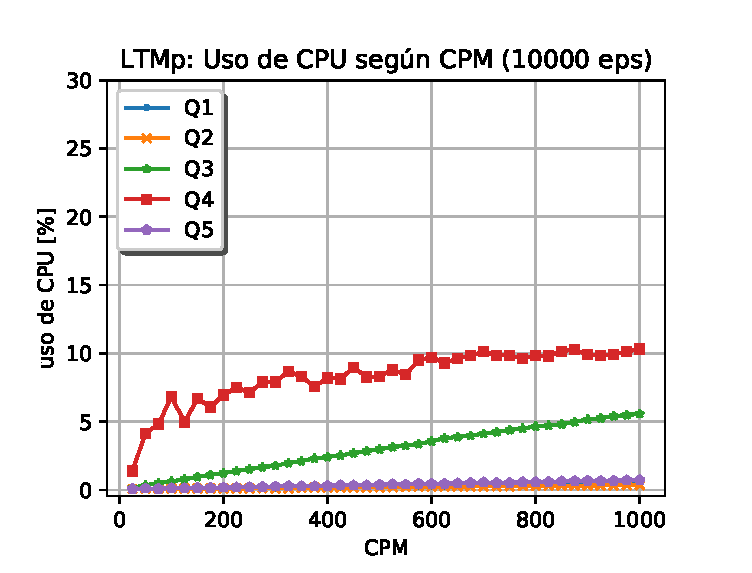
\includegraphics[width=\textwidth]{results/eff__cpu_qpm_by_query__ltm__10000_episodes.eps}
		\caption{}
		\label{result:eff__cpu_qpm_by_query__ltm__10k_episodes}
	\end{subfigure}
	~
	\begin{subfigure}[b]{0.45\textwidth}
		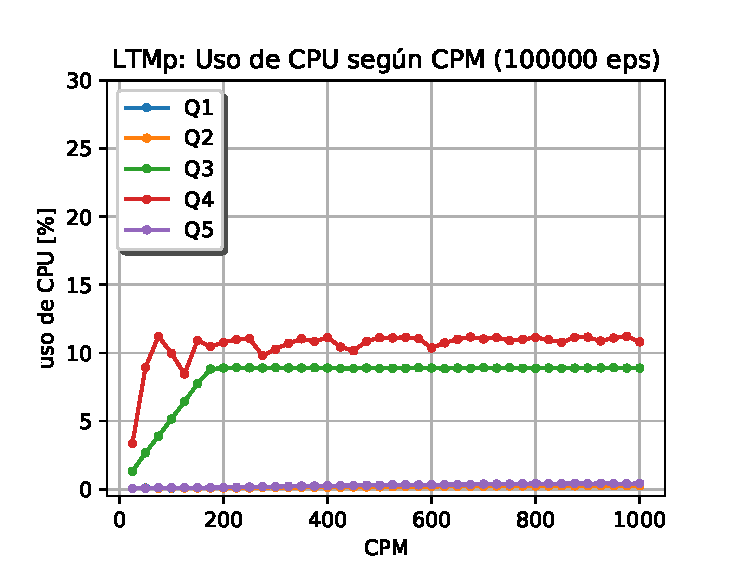
\includegraphics[width=\textwidth]{results/eff__cpu_qpm_by_query__ltm__100000_episodes.eps}
		\caption{}
		\label{result:eff__cpu_qpm_by_query__ltm__100k_episodes}
	\end{subfigure}
	~
	\begin{subfigure}[b]{0.45\textwidth}
		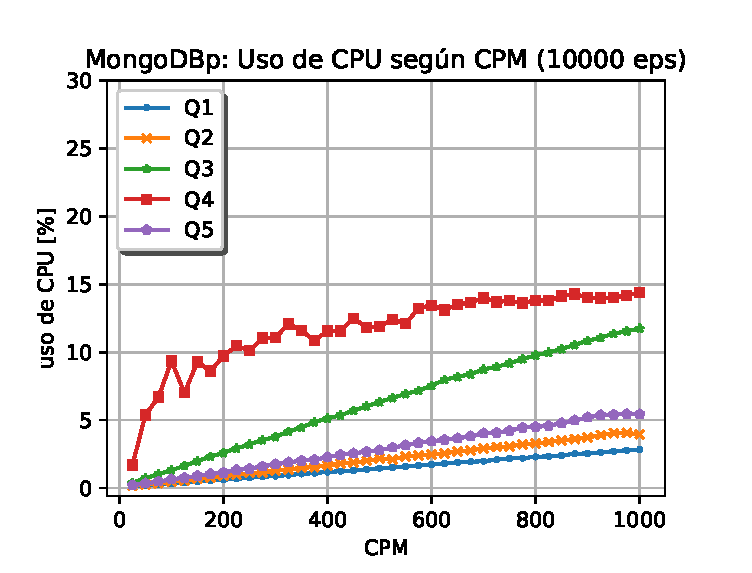
\includegraphics[width=\textwidth]{results/eff__cpu_qpm_by_query__mongo__10000_episodes.eps}
		\caption{}
		\label{result:eff__cpu_qpm_by_query__mongo__10k_episodes}
	\end{subfigure}
	~
	\begin{subfigure}[b]{0.45\textwidth}
		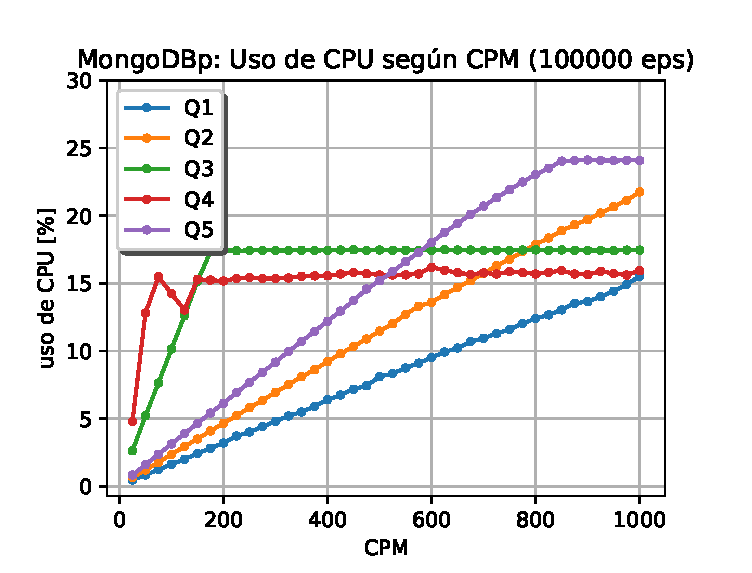
\includegraphics[width=\textwidth]{results/eff__cpu_qpm_by_query__mongo__100000_episodes.eps}
		\caption{}
		\label{result:eff__cpu_qpm_by_query__mongo__100k_episodes}
	\end{subfigure}
	~
	\begin{subfigure}[b]{0.45\textwidth}
		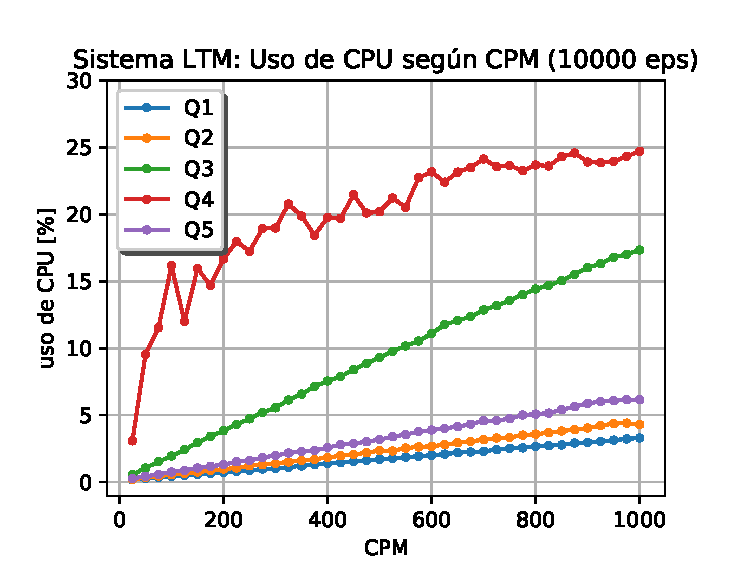
\includegraphics[width=\textwidth]{results/eff__cpu_qpm_by_query__sum__10000_episodes.eps}
		\caption{}
		\label{result:eff__cpu_qpm_by_query__sum__10k_episodes}
	\end{subfigure}
	~
	\begin{subfigure}[b]{0.45\textwidth}
		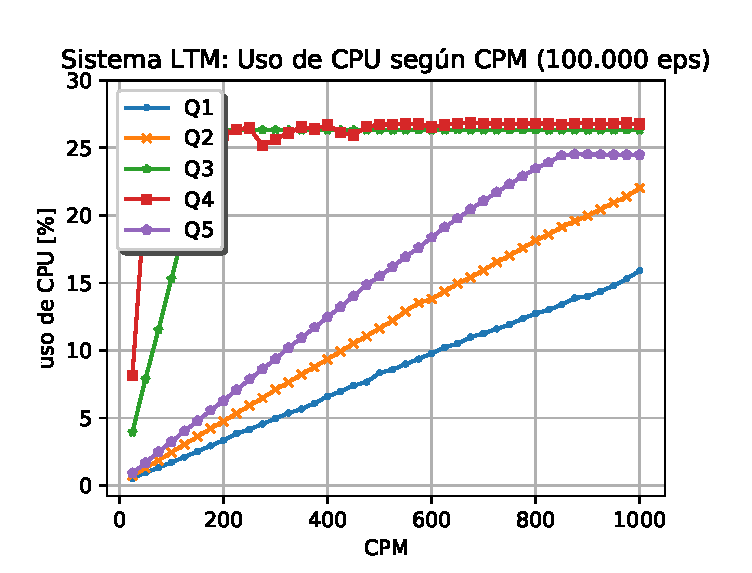
\includegraphics[width=\textwidth]{results/eff__cpu_qpm_by_query__sum__100000_episodes.eps}
		\caption{}
		\label{result:eff__cpu_qpm_by_query__sum__100k_episodes}
	\end{subfigure}
	\caption[Eficiencia: Uso de CPU según CPM bajo cantidad fija de episodios.]
	{\small Pruebas de eficiencia sobre el uso de CPU según la cantidad de CPM, bajo una cantidad fija de episodios. Se presentan 6 gráficos para distintas configuraciones, cada uno con curvas para cada consulta $Q_x$. A la izquierda hay pruebas con 10.000 episodios, a la derecha con 100.000 episodios. La primera fila muestra el uso de CPU del proceso LTMp, la segunda corresponde al uso de CPU del proceso MongoDBp y la tercera muestra la suma de ambos procesos.}
	\label{result:eff__cpu_qpm_by_query}
\end{figure}

% PEOR CASO
En el peor caso, LTPMp utiliza $\sim10\%$ del CPU y MongoDBp el $25\%$ del CPU. Es decir, MongoDBp utiliza completamente uno de los 4 núcleos disponibles, mientras que LTMp utiliza el $\sim40\%$ de otro. Sin embargo, ambos límites no se alcanzan de manera simultánea, sino que en el peor caso el sistema consume hasta un $\sim27\%$ del total del CPU. 

% MAXIMO USO DE CPU Y SATURACIÓN
El máximo uso de CPU sólo se alcanza a una tasa muy alta de CPM (cerca de 1000 CPM) o para los 100.000 episodios. En el último caso, el CPU se satura con menos de 100 CPM para las consultas $Q_3$ y $Q_4$. El resto de las consultas soportan una alta tasa de CPM sin llegar a saturar uno de los núcleos.

% COSTO DE MONGODB
Del total de CPU utilizado en cada consulta, el mayor costo se atribuye al proceso MongoDBp, el que llega a saturar el núcleo utilizado. El proceso LTMp requiere hasta un $\sim10\%$ de CPU, el que se atribuye al procesamiento de la consulta realizado por la librería de MongoDB para C++, pues la implementación del servicio bloquea el programa hasta que la consulta es respondida por la librería. Entonces, el costo de CPU se debe principalmente a la base de datos, a la librería de MongoDB y a la estructura de la consulta efectuada.

% RELACIÓN ENTRE EFICIENCIA Y ESCALABILIDAD
Finalmente, es posible ver que el costo de CPU incrementa de manera lineal  respecto a la cantidad de CPM, a excepción de $Q_4$. Además, se ve una relación directa entre el costo de CPU y el tiempo de consulta de las pruebas, presentado en los resultados de escalabilidad. Las consultas de menor costo en duración son las menos costosas en términos de CPU, mientras que $Q_3$ y $Q_4$ son más costosas en ambos ámbitos.

\todoimprove{Coma decimal, punto miles.}




\ltmconcept{Uso de CPU según CPM, revisión por cada consulta} En la Figura \ref{result:eff_cpu_qpm_by_eps__sum} se presenta un gráfico por cada consulta estudiada. En cada caso se evalúa el costo de CPU según la cantidad de CPM para distintas cantidades de episodios. Sólo se presentan los resultados para la suma de ambos procesos de interés, pues ya se ha evaluado el impacto de cada proceso por separado. Estas visualizaciones se obtienen de las mismas mediciones que las de la Figura \ref{result:eff__cpu_qpm_by_query}, pero permiten evaluar la eficiencia desde otro punto de vista.


\begin{figure}[!ht]
	\centering
	\begin{subfigure}[b]{0.45\textwidth}
		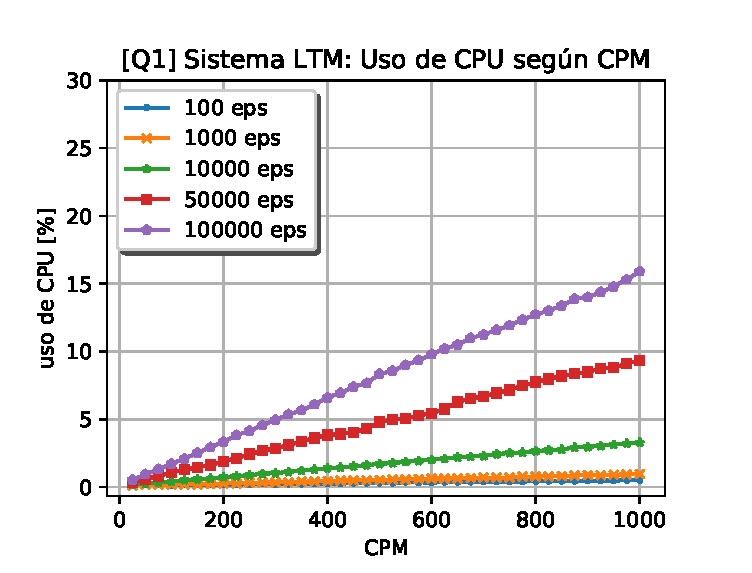
\includegraphics[width=\textwidth]{results/eff_cpu_qpm_by_eps__sum__q1.eps}
		\caption{}
		\label{result:eff_cpu_qpm_by_eps__sum__q1}
	\end{subfigure}
	~
	\begin{subfigure}[b]{0.45\textwidth}
		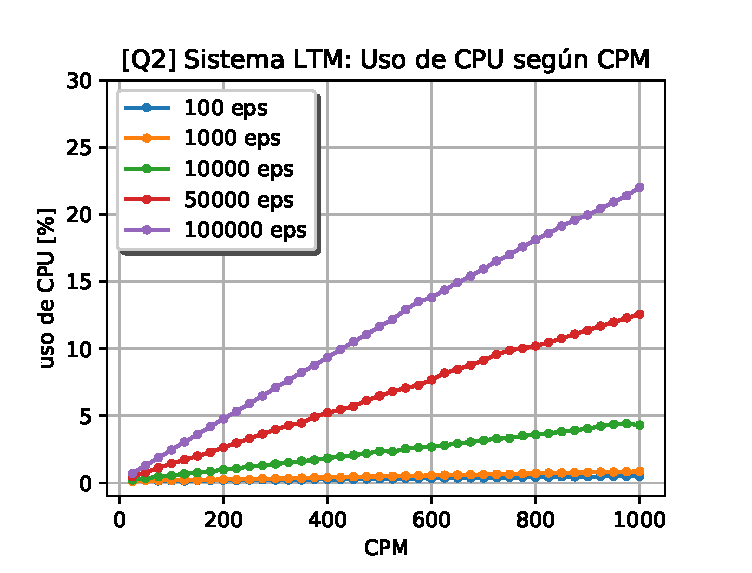
\includegraphics[width=\textwidth]{results/eff_cpu_qpm_by_eps__sum__q2.eps}
		\caption{}
		\label{result:eff_cpu_qpm_by_eps__sum__q2}
	\end{subfigure}
	~
	\begin{subfigure}[b]{0.45\textwidth}
		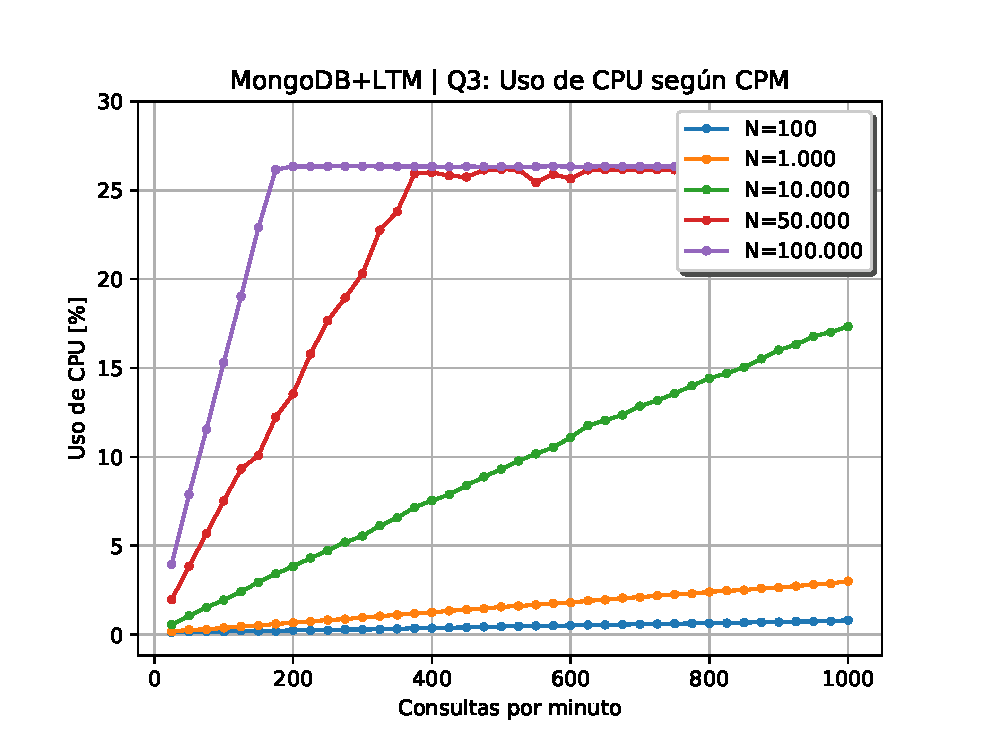
\includegraphics[width=\textwidth]{results/eff_cpu_qpm_by_eps__sum__q3.eps}
		\caption{}
		\label{result:eff_cpu_qpm_by_eps__sum__q3}
	\end{subfigure}
	~
	\begin{subfigure}[b]{0.45\textwidth}
		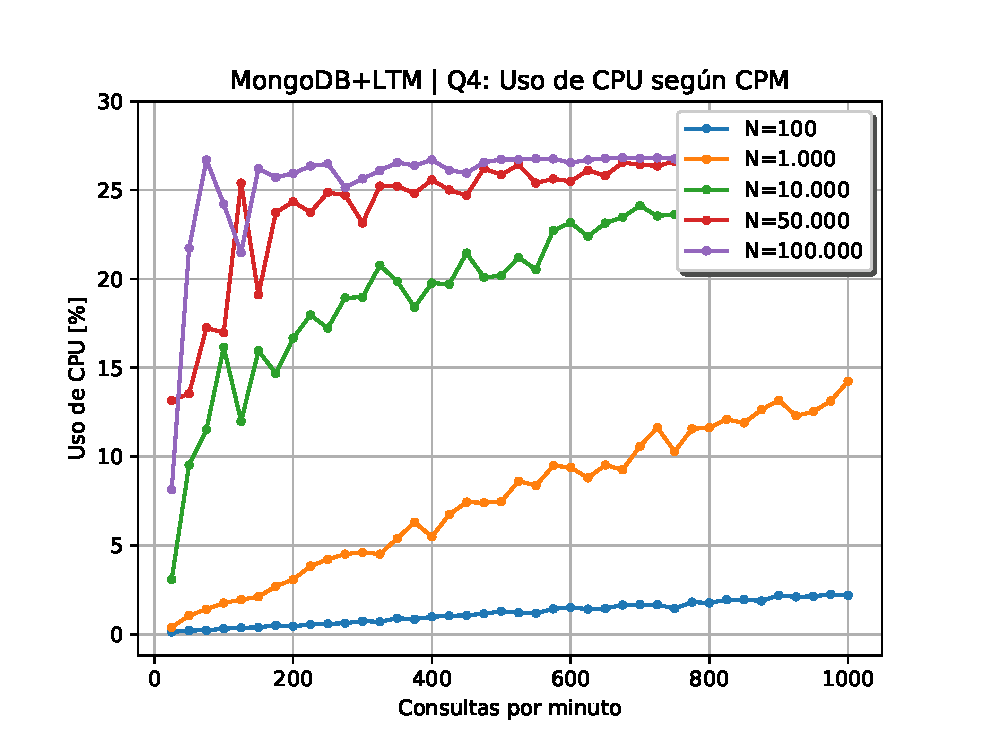
\includegraphics[width=\textwidth]{results/eff_cpu_qpm_by_eps__sum__q4.eps}
		\caption{}
		\label{result:eff_cpu_qpm_by_eps__sum__q4}
	\end{subfigure}
	~
	\begin{subfigure}[b]{0.45\textwidth}
		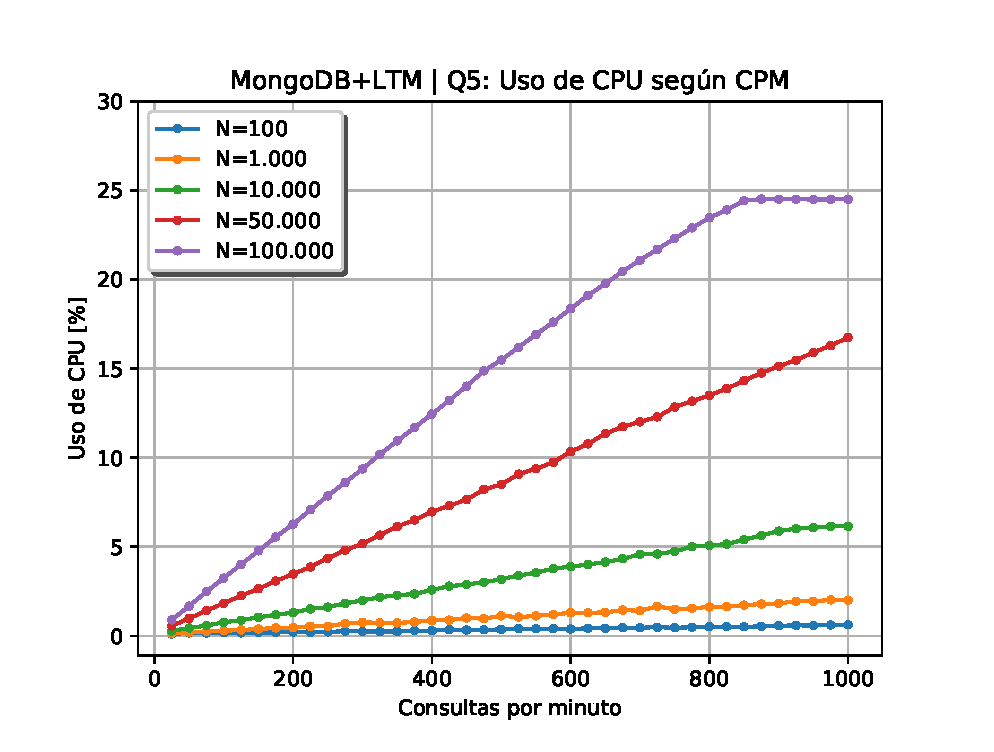
\includegraphics[width=\textwidth]{results/eff_cpu_qpm_by_eps__sum__q5.eps}
		\caption{}
		\label{result:eff_cpu_qpm_by_eps__sum__q5}
	\end{subfigure}
	\caption[Eficiencia: Uso de CPU según CPM para cada consulta de interés.]
	{\small Pruebas de eficiencia sobre el uso de CPU según la cantidad de CPM. Se presenta un gráfico para cada consulta $Q_x$. Cada uno muestra mediciones para distintas cantidades de episodios. Los valores presentados corresponden a la suma del uso de recursos por los procesos LTMp y MongoDBp.}
	\label{result:eff_cpu_qpm_by_eps__sum}
\end{figure}

Las visualizaciones reafirman que el uso de CPU para las consultas $Q_1$, $Q_2$, $Q_3$ y $Q_5$ crece de manera lineal con la cantidad de CPM y para distintas cantidades de episodios. Ya que MongoDBp sólo utiliza un núcleo del computador, tal crecimiento se estanca al saturar su capacidad.

Además, se reafirma que las consultas $Q_1$, $Q_2$ y $Q_5$ tienen bajo costo de CPU respecto a las otras consultas y escalan linealmente incluso para los 100.000 episodios. Por otro lado, $Q_3$ y $Q_4$ son consultas costosas, y particularmente, $Q_4$ ya presenta problemas a los 10.000 episodios, el equivalente a 4 meses según la estimación.


El experimento de eficiencia realizado muestra que la selección de operaciones lógicas para una consulta es importante y tiene un impacto en el desempeño del sistema. Esto puede marcar la diferencia entre la utilidad del sistema LTM y su impacto en la interacción humano-robot. 

Finalmente, se cree que la evaluación de eficiencia realizada puede ser mejorada con la consideración de hasta 300.000 episodios. Además, se puede complementar el experimento con la evaluación de la consulta de inserción y la consideración de distintos casos de uso para streams y entidades.
